\subsection{A Model for the Remote Deployment, Update, and Safe Recovery for Commercial Sensor-Based IoT Systems}
Penelitian ini menggali tantangan-tantangan khusus terkait infrastruktur yang didedikasikan untuk penyebaran dan manajemen aplikasi secara jarak jauh. Penelitian ini membahas tantangan-tantangan manajemen terkait sistem sensor IoT dan mengusulkan sebuah cara serta metodologi untuk mengatasi hal tersebut.

Penelitian ini mengimplementasikan solusi sebagai sistem infrastruktur perangkat lunak untuk produk IoT bisnis yang lengkap. Penelitian ini melakukan \textit{deployment} pada 100 perangkat penjual minuman yang tersebar di tiga lokasi. Setiap perangkat bergantung pada sensor yang memantau statusnya dan pada \textit{gateway} yang mengendalikan perilakunya. Arsitektur sistem dapat dilihat pada gambar \ref{fig:architecture-remote-deployments}.

\begin{figure}[ht]
  \centering
  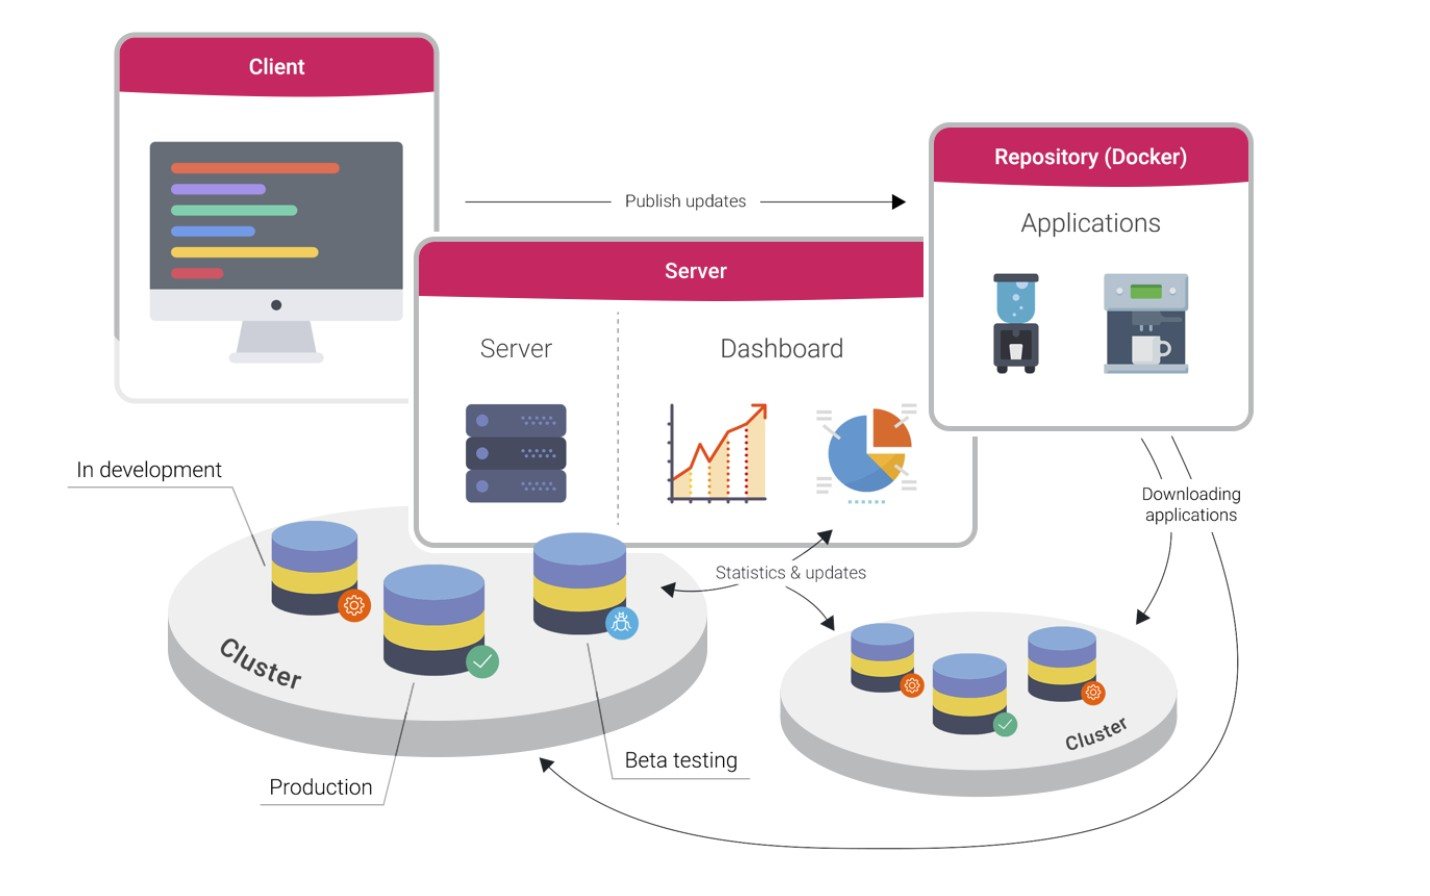
\includegraphics[width=0.8\textwidth]{resources/chapter-2/arsitektur-remote-deployment.jpg}
  \caption{Arsitektur Remote \textit{Deployment} \parencite{RemoteDeployment}}
  \label{fig:architecture-remote-deployments}
\end{figure}

Selama penelitian ini berlangsung, penelitian ini berhasil menerima 133 \textit{update} pada perangkat IoT. 80\% perangkat beroperasi tanpa gangguan selama 250 hari. Sedangkan, 20\% mengalami kegagalan akibat faktor eksternal. Dari 80\% tersebut, 30\% mengalami kegagalan pembaruan sementara akibat kapabilitas perangkat yang berkurang \parencite{RemoteDeployment}.

Solusi yang dibuat penelitian ini mengandalkan keamanan serta \textit{failsafe} yang dapat melakukan \textit{remote deployment} dengan baik serta aman sehingga dapat mendeteksi kegagalan yang terjadi pada perangkat dan melakukan \textit{recovery} dengan cepat. Berikut merupakan beberapa cara untuk melakukan \textit{remote deployment} atau seringkali disebut sebagai OTA \textit{(Over the air)}.

\begin{figure}[ht]
  \centering
  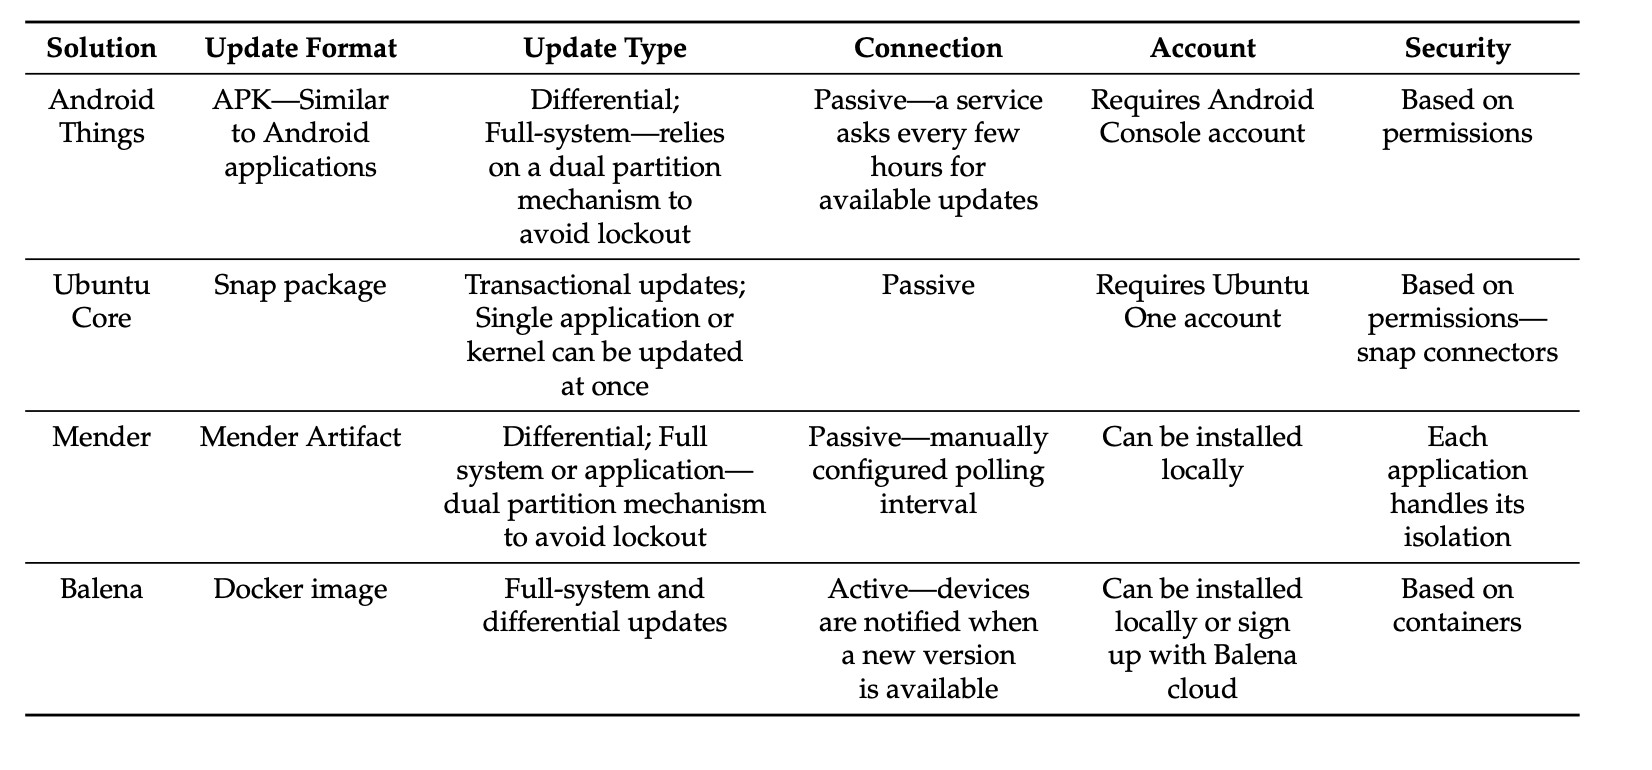
\includegraphics[width=0.8\textwidth]{resources/chapter-2/perbandingan-remote-deployment.jpg}
  \caption{Perbandingan Tata Cara \textit{Remote Deployment} \parencite{RemoteDeployment}}
  \label{fig:comparison-remote-deployments}
\end{figure}

Dapat dilihat dari gambar \ref{fig:comparison-remote-deployments} bahwa terdapat berbagai solusi untuk berbagai tipe \textit{remote deployment}. Pada kasus ini, dapat dibuat suatu cara yang mengadopsi \textit{update type} serta koneksi dari keempat tipe tersebut. Perangkat melakukan \textit{polling} kepada \textit{server} untuk mengecek apakah terdapat versi terbaru atau tidak. Selain itu, dari sisi \textit{Server} juga dapat membuat suatu notifikasi yang dapat diterima oleh perangkat jika terdapat \textit{update} baru yang siap digunakan.